\chapter{Magnolia IDE} \label{cha:ide}

This chapter will discuss the new Magnolia \gls*{ide}, the different users of the
\gls*{ide}, and their possible experiences which was under consideration when
developing the application. We will start with section \ref{sec:up} by covering
the different users that exist in \gls*{ide}s today, and how our architecture
changes this user dynamic. In sections \ref{sec:user}, and \ref{sec:module-dev},
we will cover the \gls*{ide} users and module developers of our architecture,
respectively. Specifically, we will address what the different users expect from
an \gls*{ide} in general, and what they might expect from ours. We will also
cover how some of the different modules and tools we have implemented can be
used to improve the user experience.


\section{User Perspectives} \label{sec:up}

This application has to consider different users. In \gls*{ide}'s like
Eclipse or IntelliJ, there is the primary user base, the developers
who are using the \gls*{ide} to develop, and then there are the secondary user
base, the developers whom develop modules for the \gls*{ide}.

Being the primary user base, most of the new features implemented by either
\gls*{ide} are related to the development experience. There are still changes to
that the module developers are interested in, namely \gls*{api} changes.
IntelliJ for example, lists their \textit{incompatible \gls*{api} changes}\footnote{\url{https://plugins.jetbrains.com/docs/intellij/api-changes-list-2025.html\#intellij-platform-20252}}.

Breaking changes between \gls*{ide} versions is something normal users of the
\gls*{ide} do not worry about. As usually when a new version is released, it
means more features for the developer to utilize. While module
developers have to ensure their modules still work. One of the reasons
behind \gls*{ide} version changes can break a module, is due to how
they interact with their \gls*{ide}. In IntelliJ a module is
created by implementing a Java interface for the functionality one wants. This
means a change in the interface can break the module.

A change in the \gls*{ide} architecture could break a \textit{plugin} for the
newer version of the \gls*{ide}, as with Bagge's Magnolia \gls*{ide}~\cite{baggeIde}.
While in this zero-core \gls*{ide} module developers are quite important, as they
are the ones who add the functionality to the \gls*{ide}. Therefore, the core
\gls*{api} has to be more stable, and it is by virtue of not having much
functionality.


\section{IDE users} \label{sec:user}

As mentioned in chapter \ref{cha:background}, modern \gls*{ide}s come with an
integrated module architecture. Which is used to extend/change the \gls*{ide},
from as simple as to change the theme, to more drastic changes, like changing
all key binds to \textit{vim-motions}. In any case, a user expects certain
functionality to already exist in an \gls*{ide}, like text editing. A maintainer
of a zero-core \gls*{ide} could supply modules added at compile time, meaning the
expected functionality is there out of the box, while more thematic modules
could be supplied as runtime modules. Furthermore, a maintainer can supply more
framework-like modules, which enable other modules to easier implement their
functionality.

We have implemented a few modules, some more functionality based, other more
framework-like. In the table \ref{tab:modules}, we can see these modules, their
names, and the functionality they supply.

\begin{table}[H]
  \caption{Table of framework and functionality modules}\label{tab:modules}
  \begin{center}
    \begin{tabular}[c]{l|l}
      \hline
      \multicolumn{1}{c|}{\textbf{Module name}} &
      \multicolumn{1}{c}{\textbf{Functionality}} \\
      \hline
      ide\_framework & Creates a UI framework other modules can use \\
      ide\_explorer & File explorer functionality \\
      ide\_pm & Adds the menu bar, with buttons and dropdown \\
      ide\_tabs & Responsible for the tabbing system \\
      ide\_editor & Editor \\
      ide\_fsa & Exposes File System Operations (FSA) to other modules \\
      \hline
    \end{tabular}
  \end{center}
\end{table}

\paragraph{ide\_framework} This module sets up the general \gls*{ui} layout,
which other modules depend on. In the figure \ref{fig:ideLayout}, we have laid
out the naming convention we use when referring to different \textit{places} in
the \gls*{ide}.

\begin{figure}[H]
  \centering
  \begin{tikzpicture}
  \node (window) [rectangle, draw, minimum height=7cm, minimum width=10cm] at (0, 0) {};
  \node (menu) [rectangle, draw, minimum height=0.5cm, minimum width=10cm] at (0, 3.25) {Menu};
  \node (tabs) [rectangle, draw, minimum height=0.25cm, minimum width=8cm] at (1, 2.75) {Tabs};
  \node (tab) [rectangle, draw, minimum height=0.25cm, minimum width=1cm] at (-2.5, 2.75) {Tab};
  \node (sidebar) [rectangle, draw, minimum height=6.5cm, minimum width=2cm] at (-4, -0.25) {Sidebar};
  \node (content) [rectangle, draw, minimum height=6.5cm, minimum width=8cm] at (1, -0.25) {Content};
\end{tikzpicture}
  \caption{
    Diagram of the layout of different areas in our \gls*{ide}
  }
  \label{fig:ideLayout}
\end{figure}

\paragraph{ide\_explorer} In picture \ref{pic:ideEx} we can see the
module, \textit{ide\_explorer} in action, showing the Magnolia library
visualized as a tree-like structure with collapsible folders. These folders are
rendered in the \textit{sidebar}, on the left. When we click on the
\textit{File} button in the menu, a dropdown appears, where we can click on a
button, \textit{Open Folder}, which invokes the ide\_fsa module, the module in
charge of handling file system operations, where we get in \textit{response},
all the folders and files in the path we selected. Which we transform into
\gls*{html}, and along with some \gls*{css}, we get the collapsible folders.

\begin{figure}[H]
  \centering
  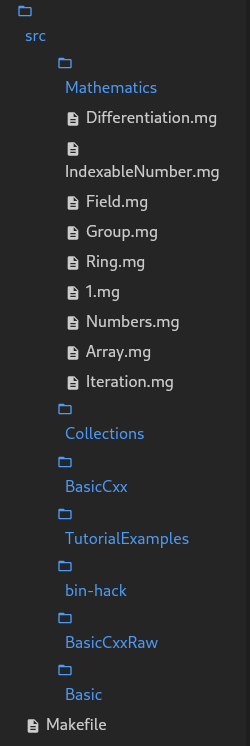
\includegraphics[height=0.5\textwidth]{ide-explorer.png}
  \caption{
    ide\_explorer module, showing the Magnolia library.
  }
  \label{pic:ideEx}
\end{figure}


\paragraph{ide\_pm} Is a module responsible for the menu bar at the top of the
\gls*{ide}. It just simplifies the creation of interactive \gls*{ui} elements
for other modules. The Module has functionality for handling dropdown menus,
which are common in \gls*{ide}-\gls*{ui}s.

\paragraph{ide\_tabs} This module handles pagination of the \gls*{ide}, where
other modules can add their own content to different tabs, that this module can
cycle through. By clicking on a file in the file explorer, a tab is made, where
the contents are managed by the \textit{ide\_editor} module.

\paragraph{ide\_editor} The editor module is coupled with the \gls*{ide}
framework, and the ide\_explorer module. We can open and edit files using the
combination of these modules. By clicking a file in the tree, we can invoke the
ide\_editor module, which invokes the ide\_tabs module, creating a tab with a
text editor in. In picture \ref{pic:editorModule} we can see this in action, as
the editor is created in the \textit{content} place, in the center of the
\gls*{ide}, along with a \textit{tab}, with the name of the file being edited as
the title of the tab.

\begin{figure}[H]
  \centering
  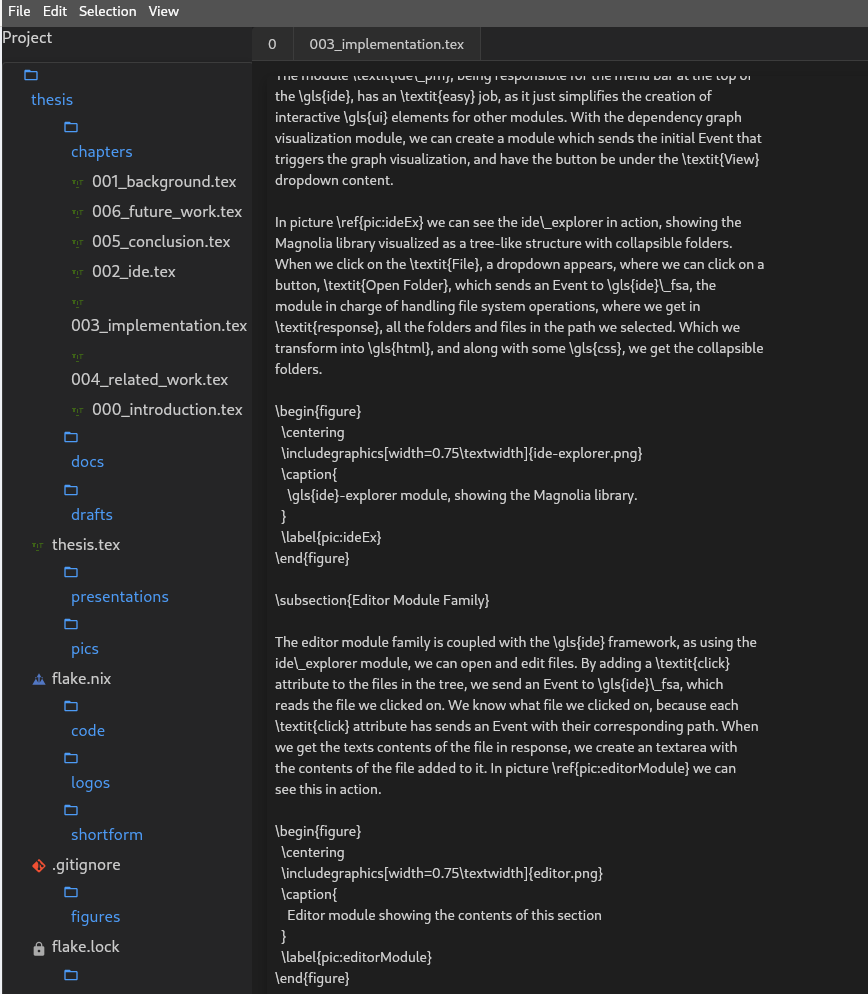
\includegraphics[width=0.5\textwidth]{editor.png}
  \caption{
    Editor module showing the contents of this section
  }
  \label{pic:editorModule}
\end{figure}

\paragraph{ide\_fsa} Since this \gls*{ide} can target different \gls*{os}es, we
need some form of \gls*{fsa}. This is achieved by our module, ide\_fsa, which
enables other modules to do file system operations without having to worry about
what \gls*{os} they are on.


\subsection{Magnolia dependency graph visualizer}

In Magnolia, as in many other languages, one cannot have a cyclic dependency.
This means that the dependency graph of a Magnolia project should be a
\gls*{dag}. And since Magnolia has such a focus on reuse, the dependency graphs
in a Magnolia project could be quite large. Which means the cycles could be
quite long, which would make resolving the cyclic dependency issue complicated.
One way to help a developer, would be to give them a tool to visualize the
dependency graph, so that they could see what modules are connected. Using the
Magnolia library as the input, we can create a visualization of the dependencies
in Magnolia. Using two modules, one for \textit{parsing} the Magnolia library,
finding all packages, and their dependencies, and another for visualizing
this.

The module responsible for rendering the graph, uses
\textit{D3}\footnote{\url{https://d3js.org/}}, a visualization library for
JavaScript. In the picture \ref{pic:magLib}, we can see the finished rendering
of the dependency graph of the Magnolia basic library. As mentioned earlier,
Magnolia has a lot of re-use, and therefore dependencies. That makes this
visualization quite \textit{noisy}, as there are a lot of crossing between the
dependencies.

\begin{figure}[H]
  \centering
  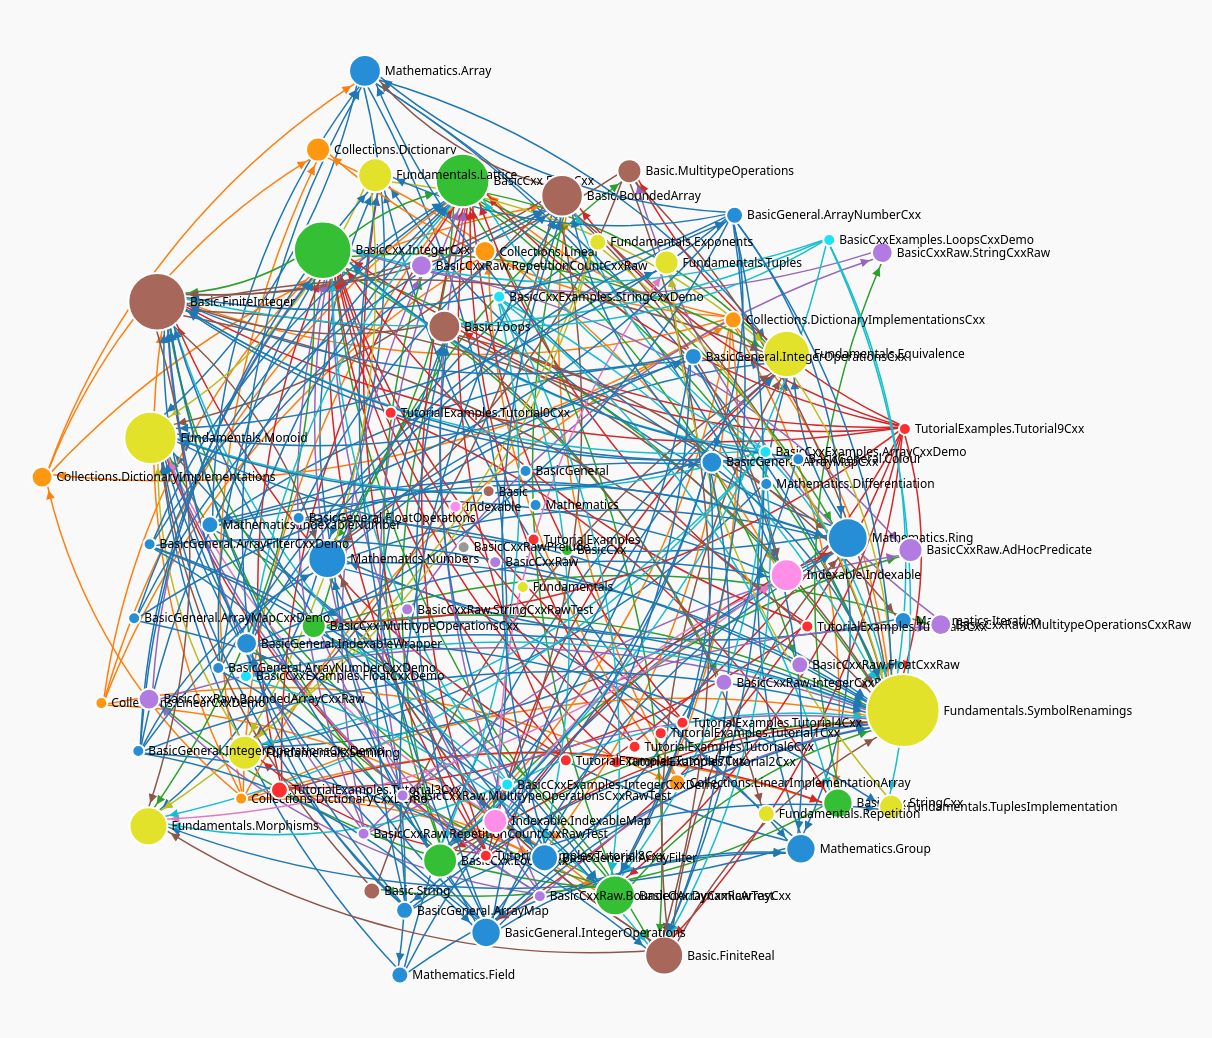
\includegraphics[width=0.75\textwidth]{magnolia-dependencies.png}
  \caption{
    A module that visualizes the dependency graph in the Magnolia basic library.
    Each colour represents a package, which contains several modules. The size
    of the nodes vary depending on the amount of dependents a module has. The
    module utilizes an external JavaScript library to create this visualization.
  }
  \label{pic:magLib}
\end{figure}

Luckily, with D3 and \gls*{css}, we can mitigate some of the noise. In the
picture \ref{pic:depCont}, we can see the control-panel that our graph module
has created. With the control panel, we can zoom in and out on the graph\footnote{This can also be done with the mouse},
and reset our view. This, along with the node size scale, scaling how big
a node is depending on how many dependents it has, ensures this visualization
tool can be used for other programming libraries, not just Magnolia.\footnote{Given a proper parser module, for the target programming language}
Furthermore, we can highlight the packages we care about, using the filter
panel the module created. In picture \ref{pic:depFil}, all the different
Magnolia packages have been detected, and their corresponding colour has been
added. We can then enable, or disable them.

\begin{figure}[H]
  \begin{subfigure}[h]{0.45\textwidth}
    \centering
    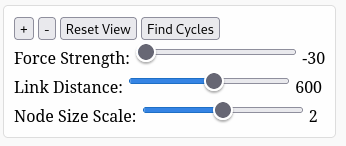
\includegraphics[width=0.85\textwidth]{dependency-viewer-controls.png}
    \caption{
      Control panel, with buttons and sliders for controlling the graph view
    }
  \label{pic:depCont}
  \end{subfigure}
  \hfill
  \begin{subfigure}[h]{0.45\textwidth}
    \centering
    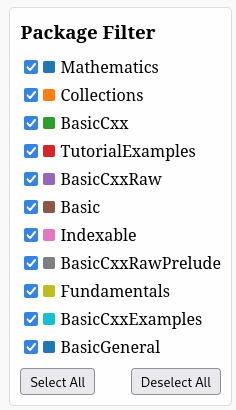
\includegraphics[height=0.8\textwidth]{dependency-viewer-filter.png}
    \caption{List of packages in the graph, that can be toggled}
    \label{pic:depFil}
  \end{subfigure}
  \caption{
    The control panel and package legend, created by the visualizer module.
  }
  \label{fig:foobarbar}
\end{figure}

In the picture \ref{pic:depDis}, we can see the graph after we have disabled all
other packages, except the \textit{Fundamentals} package.

\begin{figure}[H]
  \centering
  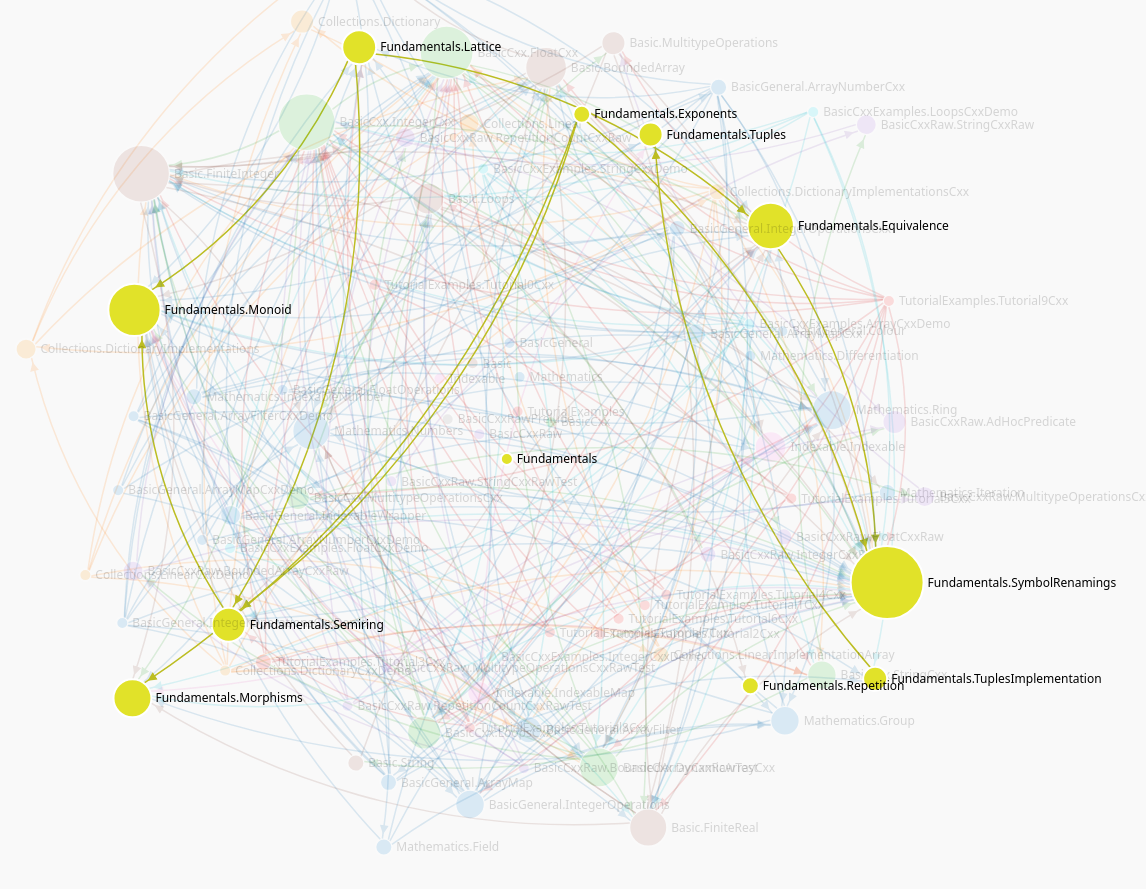
\includegraphics[width=0.75\textwidth]{magnolia-dependencies-filtered.png}
  \caption{
    A module that visualizes the dependency graph in the Magnolia basic library,
    with just the \textit{Fundamentals} package highlighted.
  }
  \label{pic:depDis}
\end{figure}


\subsection{Developer}

Most users just want an \gls*{ide}, and do not spend, nor want to spend, much
time configuring their \gls*{ide}. This can be achieved by adding the necessary
modules to qualify as an \gls*{ide} at compile time. If one is a lecturer,
teaching something that is used by a \textit{niche} programming language, the
lecturer can add the needed modules to a configuration file,
\textit{Modules.toml}, and then compile it to an \gls*{ide}. Before the \gls*{ide}
is compiled, it finds the mentioned modules in the configuration file, and
directly integrates them into the core, ensuring that the resulting binary is a
fully fledged \gls*{ide}. And then this \gls*{ide} can be distributed to the
students, who can still extend the \gls*{ide} with runtime modules at their own
digression.

\subsection{Module installer}

Module markets are an important part of the \gls*{ide} user experience. Being
able to install a module with the click of a button essential. Not having a
dedicated module market like VS Code, has not been detrimental for
Vim, as with a \textit{plugin manager}, a user can install a module by
simply supplying a URL to a GitHub repository. Similarly, we allow users to
either install modules from disk, or by supplying a URL to a GitHub repository.
In the picture \ref{pic:moduleInstaller}, we can see such a form. A user can
either install a module from disk, in which case, we simply copy the module
binary at the given path to the runtime module folder, or if a URL has been
supplied, we get the latest released binary from that GitHub repository, and
copy this binary instead.

\begin{figure}
  \centering
  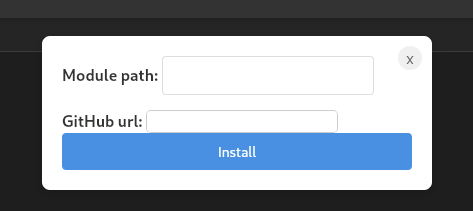
\includegraphics[width=0.50\textwidth]{module-installer.png}
  \caption{
    A module installation form, where a user can supply a path to a module on
    disk, or a URL to a GitHub repository containing the module binary.
  }
  \label{pic:moduleInstaller}
\end{figure}

\section{Module developer} \label{sec:module-dev}

Being a zero-core application; all functionality comes from modules, the module
developer experience is the most important. To achieve this, documentation is
important. If a module developer has a question about how the core might react,
it should be answered by the documentation. In Eclipse, this is in the
form of \textit{Javadoc}s, which specify, with examples how the Eclipse
runtime handles \textit{plugins}\footnote{\url{https://help.eclipse.org/latest/rtopic/org.eclipse.platform.doc.isv/reference/api/org/eclipse/core/runtime/Plugin.html}}.

The documentation for \textit{plugin} developers, in both IntelliJ and
Eclipse has to be large, due to of how \textit{plugins} interact with the
\gls*{ide}; it is a large \gls*{api}. In a zero-core \gls*{ide} it is smaller,
simply due to the fact that the core \gls*{ide} offers fewer features, as features
necessarily come from modules in a zero-core architecture.


\subsection{Language agnosticism and foreign modules}

A limiting factor in module oriented applications, is the
\textit{language barrier}. Most applications limit what language one can extend
an application with, like in VS Code, where its JavaScript/HTML/CSS. Or
IntelliJ, where one can use Java or Kotlin. But what does language agnostic
mean in the context of our modular architecture? Semantically alike modules.

Translating a module from one programming language to another should be trivial.
This is achieved by the models used in the core. The \textit{primitive} types,
are the same as in JavaScript, the notion of an empty value, numbers, strings,
lists and \textit{objects}, can be serialized/deserialized to/from any language.
So the manipulation on these types can be extracted and rewritten in another
preferred language. Therefore, to be fully language agnostic, modules should be
syntactically translatable between each other. The same two modules, one
implemented in JavaScript, the other in Rust, should be semantically the same.

Of course, this language agnosticism also extends to our libraries. Utility
functions, for manipulation the \gls*{ui} or the primitive types in our state,
should be equivalent, par for naming conventions, as this is a syntactical
difference, not semantically different.


\subsection{Module developer tools}

When developing against a module architecture, having tools to help debug issues
is useful. Common issues when developing in a modular architecture, where
modules can invoke other modules, are incorrect invocation, as in invalid
arguments or return type. Being able to manually invoke modules during runtime
is a great tool for debugging. In picture \ref{pic:eventMock} we can see this a
prototype module where module developers can manually invoke other modules.

\begin{figure}[H]
  \centering
  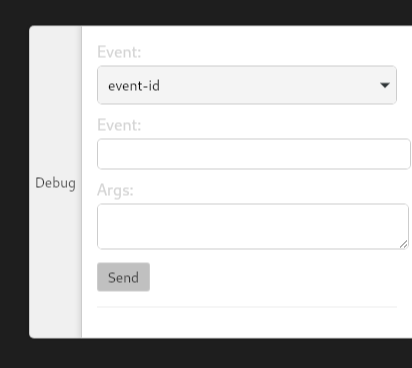
\includegraphics[width=0.5\textwidth]{event-mocking.png}
  \caption{
    Module that adds a simple pop-up menu for manually invoking other modules
  }
  \label{pic:eventMock}
\end{figure}

When mocking in \gls*{rest}-\gls*{api} development, one creates the expected
response, which is usually a \gls*{json}-file. The same is done here, where the
\textit{Args} field in this form expects the argument to be in \gls*{json}. This
is helpful, as other testing libraries, like \textit{Playwright}, does the same
and the \gls*{ide} logs the arguments in the same formatting, meaning we
can simply copy-paste the argument we want to mock from the logs, into the
field. Another helpful tool, is the one shown in the picture
\ref{pic:debugState}. Here we can see a module which visualizes the current
state of the \gls*{ide}.

\begin{figure}[H]
  \centering
  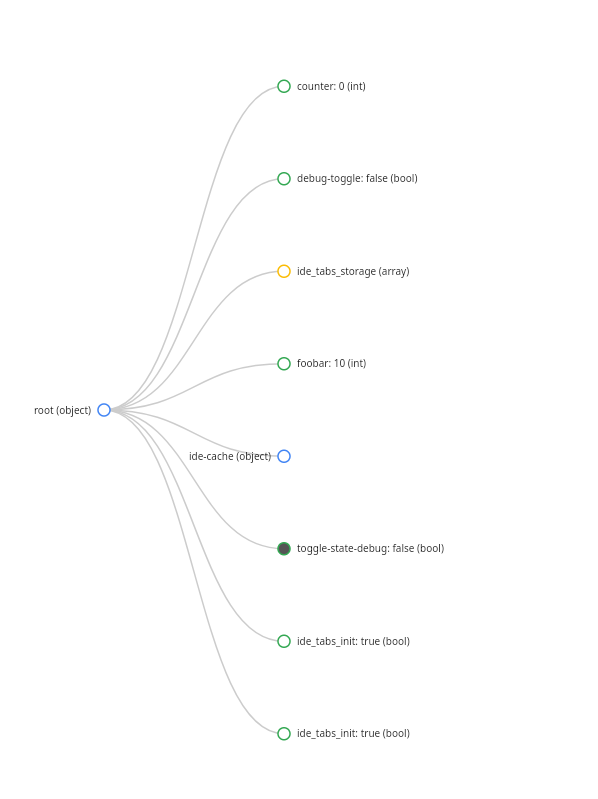
\includegraphics[width=0.75\textwidth]{debug-state.png}
  \caption{
    Module that creates a visualization of the current \gls*{ide} state. The
    visualization is made using an external JavaScript library.
  }
  \label{pic:debugState}
\end{figure}


\subsection{Module dependency visualization} \label{ssec:mdv}

When developing against a modular architecture, it is useful to be able to see
what different module families appear, and what the different dependencies
between the modules are. In picture \ref{pic:modDep} we can see the resulting
graph of the \gls*{ide} modules.

\begin{figure}[H]
  \centering
  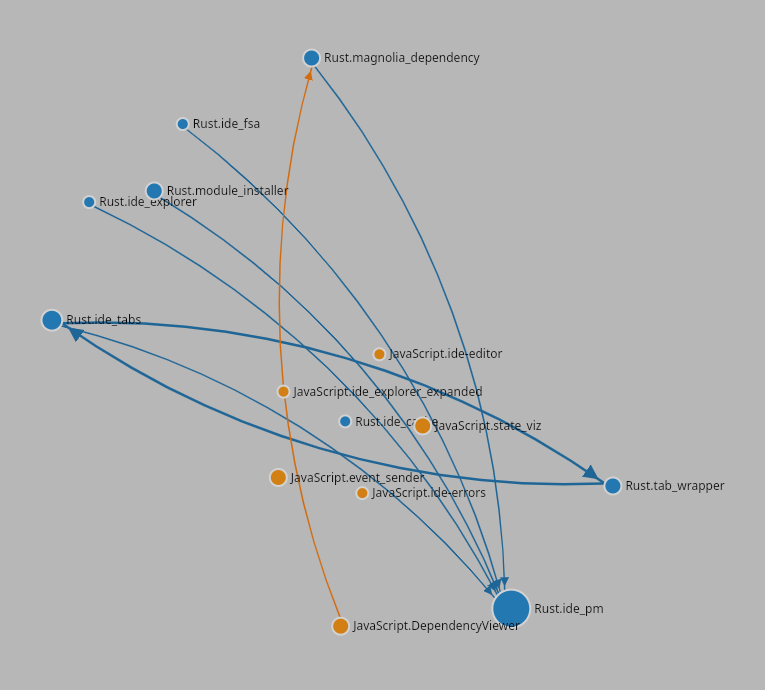
\includegraphics[width=0.75\textwidth]{module-dependencies.png}
  \caption{
    The different modules and their dependencies. Graph was created by using the
    same module shown in picture \ref{pic:magLib}.
  }
  \label{pic:modDep}
\end{figure}

